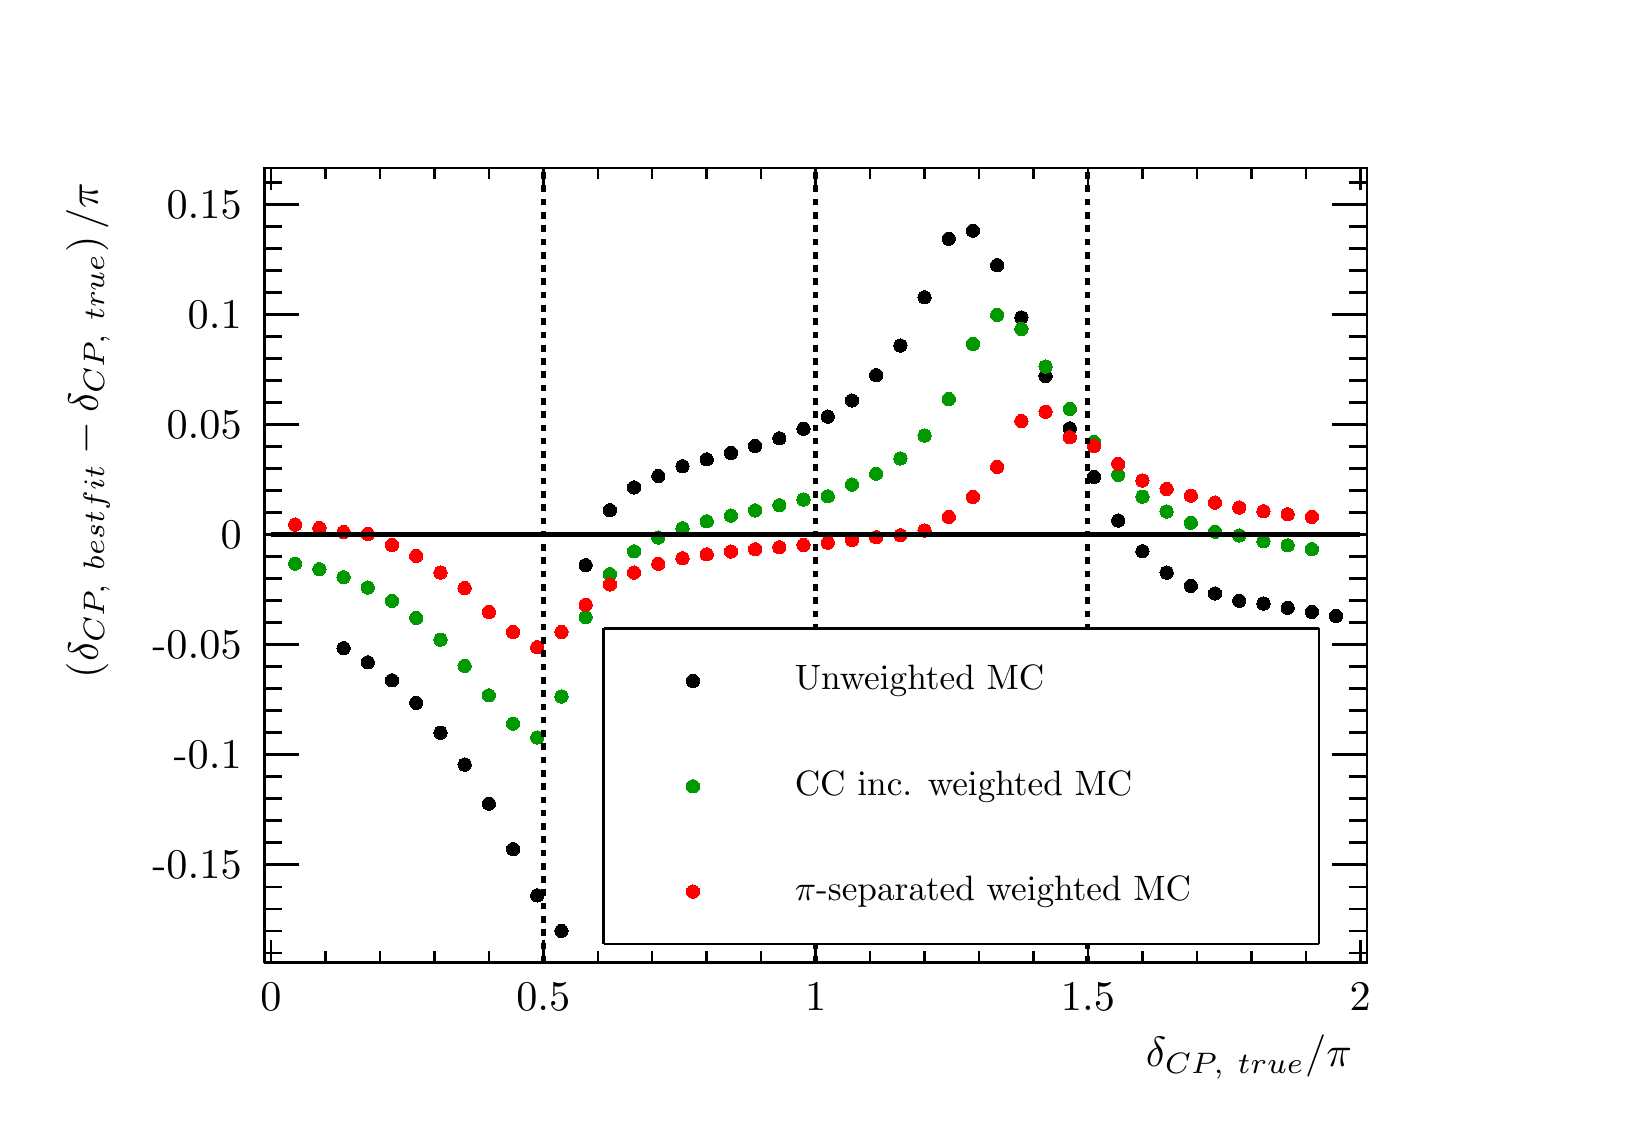
\begin{tikzpicture}
\pgfdeclareplotmark{cross} {
\pgfpathmoveto{\pgfpoint{-0.3\pgfplotmarksize}{\pgfplotmarksize}}
\pgfpathlineto{\pgfpoint{+0.3\pgfplotmarksize}{\pgfplotmarksize}}
\pgfpathlineto{\pgfpoint{+0.3\pgfplotmarksize}{0.3\pgfplotmarksize}}
\pgfpathlineto{\pgfpoint{+1\pgfplotmarksize}{0.3\pgfplotmarksize}}
\pgfpathlineto{\pgfpoint{+1\pgfplotmarksize}{-0.3\pgfplotmarksize}}
\pgfpathlineto{\pgfpoint{+0.3\pgfplotmarksize}{-0.3\pgfplotmarksize}}
\pgfpathlineto{\pgfpoint{+0.3\pgfplotmarksize}{-1.\pgfplotmarksize}}
\pgfpathlineto{\pgfpoint{-0.3\pgfplotmarksize}{-1.\pgfplotmarksize}}
\pgfpathlineto{\pgfpoint{-0.3\pgfplotmarksize}{-0.3\pgfplotmarksize}}
\pgfpathlineto{\pgfpoint{-1.\pgfplotmarksize}{-0.3\pgfplotmarksize}}
\pgfpathlineto{\pgfpoint{-1.\pgfplotmarksize}{0.3\pgfplotmarksize}}
\pgfpathlineto{\pgfpoint{-0.3\pgfplotmarksize}{0.3\pgfplotmarksize}}
\pgfpathclose
\pgfusepathqstroke
}
\pgfdeclareplotmark{cross*} {
\pgfpathmoveto{\pgfpoint{-0.3\pgfplotmarksize}{\pgfplotmarksize}}
\pgfpathlineto{\pgfpoint{+0.3\pgfplotmarksize}{\pgfplotmarksize}}
\pgfpathlineto{\pgfpoint{+0.3\pgfplotmarksize}{0.3\pgfplotmarksize}}
\pgfpathlineto{\pgfpoint{+1\pgfplotmarksize}{0.3\pgfplotmarksize}}
\pgfpathlineto{\pgfpoint{+1\pgfplotmarksize}{-0.3\pgfplotmarksize}}
\pgfpathlineto{\pgfpoint{+0.3\pgfplotmarksize}{-0.3\pgfplotmarksize}}
\pgfpathlineto{\pgfpoint{+0.3\pgfplotmarksize}{-1.\pgfplotmarksize}}
\pgfpathlineto{\pgfpoint{-0.3\pgfplotmarksize}{-1.\pgfplotmarksize}}
\pgfpathlineto{\pgfpoint{-0.3\pgfplotmarksize}{-0.3\pgfplotmarksize}}
\pgfpathlineto{\pgfpoint{-1.\pgfplotmarksize}{-0.3\pgfplotmarksize}}
\pgfpathlineto{\pgfpoint{-1.\pgfplotmarksize}{0.3\pgfplotmarksize}}
\pgfpathlineto{\pgfpoint{-0.3\pgfplotmarksize}{0.3\pgfplotmarksize}}
\pgfpathclose
\pgfusepathqfillstroke
}
\pgfdeclareplotmark{newstar} {
\pgfpathmoveto{\pgfqpoint{0pt}{\pgfplotmarksize}}
\pgfpathlineto{\pgfqpointpolar{44}{0.5\pgfplotmarksize}}
\pgfpathlineto{\pgfqpointpolar{18}{\pgfplotmarksize}}
\pgfpathlineto{\pgfqpointpolar{-20}{0.5\pgfplotmarksize}}
\pgfpathlineto{\pgfqpointpolar{-54}{\pgfplotmarksize}}
\pgfpathlineto{\pgfqpointpolar{-90}{0.5\pgfplotmarksize}}
\pgfpathlineto{\pgfqpointpolar{234}{\pgfplotmarksize}}
\pgfpathlineto{\pgfqpointpolar{198}{0.5\pgfplotmarksize}}
\pgfpathlineto{\pgfqpointpolar{162}{\pgfplotmarksize}}
\pgfpathlineto{\pgfqpointpolar{134}{0.5\pgfplotmarksize}}
\pgfpathclose
\pgfusepathqstroke
}
\pgfdeclareplotmark{newstar*} {
\pgfpathmoveto{\pgfqpoint{0pt}{\pgfplotmarksize}}
\pgfpathlineto{\pgfqpointpolar{44}{0.5\pgfplotmarksize}}
\pgfpathlineto{\pgfqpointpolar{18}{\pgfplotmarksize}}
\pgfpathlineto{\pgfqpointpolar{-20}{0.5\pgfplotmarksize}}
\pgfpathlineto{\pgfqpointpolar{-54}{\pgfplotmarksize}}
\pgfpathlineto{\pgfqpointpolar{-90}{0.5\pgfplotmarksize}}
\pgfpathlineto{\pgfqpointpolar{234}{\pgfplotmarksize}}
\pgfpathlineto{\pgfqpointpolar{198}{0.5\pgfplotmarksize}}
\pgfpathlineto{\pgfqpointpolar{162}{\pgfplotmarksize}}
\pgfpathlineto{\pgfqpointpolar{134}{0.5\pgfplotmarksize}}
\pgfpathclose
\pgfusepathqfillstroke
}
\definecolor{c}{rgb}{1,1,1};
\draw [color=c, fill=c] (0,0) rectangle (20,13.639);
\draw [color=c, fill=c] (3,1.77307) rectangle (17,11.8659);
\definecolor{c}{rgb}{0,0,0};
\draw [c,line width=0.9] (3,1.77307) -- (3,11.8659) -- (17,11.8659) -- (17,1.77307) -- (3,1.77307);
\definecolor{c}{rgb}{1,1,1};
\draw [color=c, fill=c] (3,1.77307) rectangle (17,11.8659);
\definecolor{c}{rgb}{0,0,0};
\draw [c,line width=0.9] (3,1.77307) -- (3,11.8659) -- (17,11.8659) -- (17,1.77307) -- (3,1.77307);
\draw [c,line width=0.9] (3,1.77307) -- (17,1.77307);
\draw [c,line width=0.9] (3.083,2.05948) -- (3.083,1.77307);
\draw [c,line width=0.9] (3.7747,1.91628) -- (3.7747,1.77307);
\draw [c,line width=0.9] (4.4664,1.91628) -- (4.4664,1.77307);
\draw [c,line width=0.9] (5.1581,1.91628) -- (5.1581,1.77307);
\draw [c,line width=0.9] (5.8498,1.91628) -- (5.8498,1.77307);
\draw [c,line width=0.9] (6.5415,2.05948) -- (6.5415,1.77307);
\draw [c,line width=0.9] (7.2332,1.91628) -- (7.2332,1.77307);
\draw [c,line width=0.9] (7.9249,1.91628) -- (7.9249,1.77307);
\draw [c,line width=0.9] (8.6166,1.91628) -- (8.6166,1.77307);
\draw [c,line width=0.9] (9.3083,1.91628) -- (9.3083,1.77307);
\draw [c,line width=0.9] (10,2.05948) -- (10,1.77307);
\draw [c,line width=0.9] (10.6917,1.91628) -- (10.6917,1.77307);
\draw [c,line width=0.9] (11.3834,1.91628) -- (11.3834,1.77307);
\draw [c,line width=0.9] (12.0751,1.91628) -- (12.0751,1.77307);
\draw [c,line width=0.9] (12.7668,1.91628) -- (12.7668,1.77307);
\draw [c,line width=0.9] (13.4585,2.05948) -- (13.4585,1.77307);
\draw [c,line width=0.9] (14.1502,1.91628) -- (14.1502,1.77307);
\draw [c,line width=0.9] (14.8419,1.91628) -- (14.8419,1.77307);
\draw [c,line width=0.9] (15.5336,1.91628) -- (15.5336,1.77307);
\draw [c,line width=0.9] (16.2253,1.91628) -- (16.2253,1.77307);
\draw [c,line width=0.9] (16.917,2.05948) -- (16.917,1.77307);
\draw [c,line width=0.9] (3.083,2.05948) -- (3.083,1.77307);
\draw [c,line width=0.9] (16.917,2.05948) -- (16.917,1.77307);
\draw [anchor=base] (3.083,1.15931) node[scale=1.52731, color=c, rotate=0]{0};
\draw [anchor=base] (6.5415,1.15931) node[scale=1.52731, color=c, rotate=0]{0.5};
\draw [anchor=base] (10,1.15931) node[scale=1.52731, color=c, rotate=0]{1};
\draw [anchor=base] (13.4585,1.15931) node[scale=1.52731, color=c, rotate=0]{1.5};
\draw [anchor=base] (16.917,1.15931) node[scale=1.52731, color=c, rotate=0]{2};
\draw [anchor= east] (17,0.572837) node[scale=1.52731, color=c, rotate=0]{$ \delta_{CP,~\text{true}} / \pi$};
\draw [c,line width=0.9] (3,11.8659) -- (17,11.8659);
\draw [c,line width=0.9] (3.083,11.5795) -- (3.083,11.8659);
\draw [c,line width=0.9] (3.7747,11.7227) -- (3.7747,11.8659);
\draw [c,line width=0.9] (4.4664,11.7227) -- (4.4664,11.8659);
\draw [c,line width=0.9] (5.1581,11.7227) -- (5.1581,11.8659);
\draw [c,line width=0.9] (5.8498,11.7227) -- (5.8498,11.8659);
\draw [c,line width=0.9] (6.5415,11.5795) -- (6.5415,11.8659);
\draw [c,line width=0.9] (7.2332,11.7227) -- (7.2332,11.8659);
\draw [c,line width=0.9] (7.9249,11.7227) -- (7.9249,11.8659);
\draw [c,line width=0.9] (8.6166,11.7227) -- (8.6166,11.8659);
\draw [c,line width=0.9] (9.3083,11.7227) -- (9.3083,11.8659);
\draw [c,line width=0.9] (10,11.5795) -- (10,11.8659);
\draw [c,line width=0.9] (10.6917,11.7227) -- (10.6917,11.8659);
\draw [c,line width=0.9] (11.3834,11.7227) -- (11.3834,11.8659);
\draw [c,line width=0.9] (12.0751,11.7227) -- (12.0751,11.8659);
\draw [c,line width=0.9] (12.7668,11.7227) -- (12.7668,11.8659);
\draw [c,line width=0.9] (13.4585,11.5795) -- (13.4585,11.8659);
\draw [c,line width=0.9] (14.1502,11.7227) -- (14.1502,11.8659);
\draw [c,line width=0.9] (14.8419,11.7227) -- (14.8419,11.8659);
\draw [c,line width=0.9] (15.5336,11.7227) -- (15.5336,11.8659);
\draw [c,line width=0.9] (16.2253,11.7227) -- (16.2253,11.8659);
\draw [c,line width=0.9] (16.917,11.5795) -- (16.917,11.8659);
\draw [c,line width=0.9] (3.083,11.5795) -- (3.083,11.8659);
\draw [c,line width=0.9] (16.917,11.5795) -- (16.917,11.8659);
\draw [c,line width=0.9] (3,1.77307) -- (3,11.8659);
\draw [c,line width=0.9] (3.444,3.01526) -- (3,3.01526);
\draw [c,line width=0.9] (3.222,3.29475) -- (3,3.29475);
\draw [c,line width=0.9] (3.222,3.57425) -- (3,3.57425);
\draw [c,line width=0.9] (3.222,3.85374) -- (3,3.85374);
\draw [c,line width=0.9] (3.222,4.13324) -- (3,4.13324);
\draw [c,line width=0.9] (3.444,4.41273) -- (3,4.41273);
\draw [c,line width=0.9] (3.222,4.69222) -- (3,4.69222);
\draw [c,line width=0.9] (3.222,4.97172) -- (3,4.97172);
\draw [c,line width=0.9] (3.222,5.25121) -- (3,5.25121);
\draw [c,line width=0.9] (3.222,5.53071) -- (3,5.53071);
\draw [c,line width=0.9] (3.444,5.8102) -- (3,5.8102);
\draw [c,line width=0.9] (3.222,6.08969) -- (3,6.08969);
\draw [c,line width=0.9] (3.222,6.36919) -- (3,6.36919);
\draw [c,line width=0.9] (3.222,6.64868) -- (3,6.64868);
\draw [c,line width=0.9] (3.222,6.92818) -- (3,6.92818);
\draw [c,line width=0.9] (3.444,7.20767) -- (3,7.20767);
\draw [c,line width=0.9] (3.222,7.48716) -- (3,7.48716);
\draw [c,line width=0.9] (3.222,7.76666) -- (3,7.76666);
\draw [c,line width=0.9] (3.222,8.04615) -- (3,8.04615);
\draw [c,line width=0.9] (3.222,8.32565) -- (3,8.32565);
\draw [c,line width=0.9] (3.444,8.60514) -- (3,8.60514);
\draw [c,line width=0.9] (3.222,8.88463) -- (3,8.88463);
\draw [c,line width=0.9] (3.222,9.16413) -- (3,9.16413);
\draw [c,line width=0.9] (3.222,9.44362) -- (3,9.44362);
\draw [c,line width=0.9] (3.222,9.72312) -- (3,9.72312);
\draw [c,line width=0.9] (3.444,10.0026) -- (3,10.0026);
\draw [c,line width=0.9] (3.222,10.2821) -- (3,10.2821);
\draw [c,line width=0.9] (3.222,10.5616) -- (3,10.5616);
\draw [c,line width=0.9] (3.222,10.8411) -- (3,10.8411);
\draw [c,line width=0.9] (3.222,11.1206) -- (3,11.1206);
\draw [c,line width=0.9] (3.444,11.4001) -- (3,11.4001);
\draw [c,line width=0.9] (3.444,3.01526) -- (3,3.01526);
\draw [c,line width=0.9] (3.222,2.73577) -- (3,2.73577);
\draw [c,line width=0.9] (3.222,2.45627) -- (3,2.45627);
\draw [c,line width=0.9] (3.222,2.17678) -- (3,2.17678);
\draw [c,line width=0.9] (3.222,1.89729) -- (3,1.89729);
\draw [c,line width=0.9] (3.444,11.4001) -- (3,11.4001);
\draw [c,line width=0.9] (3.222,11.6796) -- (3,11.6796);
\draw [anchor= east] (2.9,3.01526) node[scale=1.52731, color=c, rotate=0]{-0.15};
\draw [anchor= east] (2.9,4.41273) node[scale=1.52731, color=c, rotate=0]{-0.1};
\draw [anchor= east] (2.9,5.8102) node[scale=1.52731, color=c, rotate=0]{-0.05};
\draw [anchor= east] (2.9,7.20767) node[scale=1.52731, color=c, rotate=0]{0};
\draw [anchor= east] (2.9,8.60514) node[scale=1.52731, color=c, rotate=0]{0.05};
\draw [anchor= east] (2.9,10.0026) node[scale=1.52731, color=c, rotate=0]{0.1};
\draw [anchor= east] (2.9,11.4001) node[scale=1.52731, color=c, rotate=0]{0.15};
\draw [anchor= east] (0.76,11.8659) node[scale=1.52731, color=c, rotate=90]{$\left( \delta_{CP,~\text{best fit}} - \delta_{CP,~\text{true}} \right) / \pi$};
\draw [c,line width=0.9] (17,1.77307) -- (17,11.8659);
\draw [c,line width=0.9] (16.556,3.01526) -- (17,3.01526);
\draw [c,line width=0.9] (16.778,3.29475) -- (17,3.29475);
\draw [c,line width=0.9] (16.778,3.57425) -- (17,3.57425);
\draw [c,line width=0.9] (16.778,3.85374) -- (17,3.85374);
\draw [c,line width=0.9] (16.778,4.13324) -- (17,4.13324);
\draw [c,line width=0.9] (16.556,4.41273) -- (17,4.41273);
\draw [c,line width=0.9] (16.778,4.69222) -- (17,4.69222);
\draw [c,line width=0.9] (16.778,4.97172) -- (17,4.97172);
\draw [c,line width=0.9] (16.778,5.25121) -- (17,5.25121);
\draw [c,line width=0.9] (16.778,5.53071) -- (17,5.53071);
\draw [c,line width=0.9] (16.556,5.8102) -- (17,5.8102);
\draw [c,line width=0.9] (16.778,6.08969) -- (17,6.08969);
\draw [c,line width=0.9] (16.778,6.36919) -- (17,6.36919);
\draw [c,line width=0.9] (16.778,6.64868) -- (17,6.64868);
\draw [c,line width=0.9] (16.778,6.92818) -- (17,6.92818);
\draw [c,line width=0.9] (16.556,7.20767) -- (17,7.20767);
\draw [c,line width=0.9] (16.778,7.48716) -- (17,7.48716);
\draw [c,line width=0.9] (16.778,7.76666) -- (17,7.76666);
\draw [c,line width=0.9] (16.778,8.04615) -- (17,8.04615);
\draw [c,line width=0.9] (16.778,8.32565) -- (17,8.32565);
\draw [c,line width=0.9] (16.556,8.60514) -- (17,8.60514);
\draw [c,line width=0.9] (16.778,8.88463) -- (17,8.88463);
\draw [c,line width=0.9] (16.778,9.16413) -- (17,9.16413);
\draw [c,line width=0.9] (16.778,9.44362) -- (17,9.44362);
\draw [c,line width=0.9] (16.778,9.72312) -- (17,9.72312);
\draw [c,line width=0.9] (16.556,10.0026) -- (17,10.0026);
\draw [c,line width=0.9] (16.778,10.2821) -- (17,10.2821);
\draw [c,line width=0.9] (16.778,10.5616) -- (17,10.5616);
\draw [c,line width=0.9] (16.778,10.8411) -- (17,10.8411);
\draw [c,line width=0.9] (16.778,11.1206) -- (17,11.1206);
\draw [c,line width=0.9] (16.556,11.4001) -- (17,11.4001);
\draw [c,line width=0.9] (16.556,3.01526) -- (17,3.01526);
\draw [c,line width=0.9] (16.778,2.73577) -- (17,2.73577);
\draw [c,line width=0.9] (16.778,2.45627) -- (17,2.45627);
\draw [c,line width=0.9] (16.778,2.17678) -- (17,2.17678);
\draw [c,line width=0.9] (16.778,1.89729) -- (17,1.89729);
\draw [c,line width=0.9] (16.556,11.4001) -- (17,11.4001);
\draw [c,line width=0.9] (16.778,11.6796) -- (17,11.6796);
\foreach \P in {(4.00527,5.76608), (4.31269,5.58593), (4.62011,5.35762), (4.92754,5.07113), (5.23496,4.69224), (5.54238,4.2865), (5.8498,3.79035), (6.15722,3.21289), (6.46465,2.62632), (6.77207,2.17554), (7.07949,6.81969), (7.38691,7.51835),
 (7.69433,7.8076), (8.00176,7.95227), (8.30918,8.07628), (8.6166,8.16367), (8.92402,8.24539), (9.23145,8.33282), (9.53887,8.43079), (9.84629,8.55175), (10.1537,8.70606), (10.4611,8.91108), (10.7686,9.23315), (11.076,9.60927), (11.3834,10.2215),
 (11.6908,10.9653), (11.9982,11.067), (12.3057,10.6293), (12.6131,9.96566), (12.9205,9.22254), (13.2279,8.55726), (13.5354,7.94024), (13.8428,7.38589), (14.1502,6.9972), (14.4576,6.72496), (14.765,6.55773), (15.0725,6.46015), (15.3799,6.36803),
 (15.6873,6.33215), (15.9947,6.27896), (16.3022,6.22681), (16.6096,6.17509)}{\draw[mark options={color=c,fill=c},mark size=2.402402pt, line width=0.000000pt, mark=*] plot coordinates {\P};}
\definecolor{c}{rgb}{0,0.6,0};
\foreach \P in {(3.39043,6.83849), (3.69785,6.76932), (4.00527,6.66734), (4.31269,6.53591), (4.62011,6.36735), (4.92754,6.14991), (5.23496,5.87372), (5.54238,5.54092), (5.8498,5.16671), (6.15722,4.80709), (6.46465,4.63155), (6.77207,5.152),
 (7.07949,6.16016), (7.38691,6.70512), (7.69433,6.99567), (8.00176,7.17025), (8.30918,7.28831), (8.6166,7.37636), (8.92402,7.44904), (9.23145,7.51528), (9.53887,7.58123), (9.84629,7.65325), (10.1537,7.69432), (10.4611,7.84311), (10.7686,7.98133),
 (11.076,8.17501), (11.3834,8.46526), (11.6908,8.92944), (11.9982,9.62928), (12.3057,9.99905), (12.6131,9.82012), (12.9205,9.34211), (13.2279,8.80542), (13.5354,8.38422), (13.8428,7.96675), (14.1502,7.68989), (14.4576,7.50099), (14.765,7.35856),
 (15.0725,7.24397), (15.3799,7.19656), (15.6873,7.12281), (15.9947,7.07175), (16.3022,7.02329)}{\draw[mark options={color=c,fill=c},mark size=2.402402pt, line width=0.000000pt, mark=*] plot coordinates {\P};}
\definecolor{c}{rgb}{1,0,0};
\foreach \P in {(3.39043,7.33439), (3.69785,7.29285), (4.00527,7.24017), (4.31269,7.21531), (4.62011,7.07725), (4.92754,6.93649), (5.23496,6.72501), (5.54238,6.52881), (5.8498,6.22528), (6.15722,5.97), (6.46465,5.7781), (6.77207,5.97155),
 (7.07949,6.31699), (7.38691,6.57504), (7.69433,6.72553), (8.00176,6.83713), (8.30918,6.907), (8.6166,6.95751), (8.92402,6.99286), (9.23145,7.02227), (9.53887,7.04727), (9.84629,7.07634), (10.1537,7.10567), (10.4611,7.1385), (10.7686,7.17467),
 (11.076,7.19987), (11.3834,7.25978), (11.6908,7.43183), (11.9982,7.68764), (12.3057,8.06846), (12.6131,8.65059), (12.9205,8.76876), (13.2279,8.44453), (13.5354,8.33363), (13.8428,8.10581), (14.1502,7.89459), (14.4576,7.78799), (14.765,7.70262),
 (15.0725,7.61392), (15.3799,7.55126), (15.6873,7.50494), (15.9947,7.4665), (16.3022,7.43293)}{\draw[mark options={color=c,fill=c},mark size=2.402402pt, line width=0.000000pt, mark=*] plot coordinates {\P};}
\definecolor{c}{rgb}{1,1,1};
\draw [color=c, fill=c] (2,12.8206) rectangle (18,13.5708);
\definecolor{c}{rgb}{0,0,0};
\draw [c,line width=1.8] (3.083,7.20767) -- (16.917,7.20767);
\draw [c,dash pattern=on 2.40pt off 2.40pt ,line width=1.8] (6.5415,1.77307) -- (6.5415,11.8659);
\draw [c,dash pattern=on 2.40pt off 2.40pt ,line width=1.8] (10,1.77307) -- (10,11.8659);
\draw [c,dash pattern=on 2.40pt off 2.40pt ,line width=1.8] (13.4585,1.77307) -- (13.4585,11.8659);
\definecolor{c}{rgb}{1,1,1};
\draw [color=c, fill=c] (7.30659,2.00573) rectangle (16.3897,6.01719);
\definecolor{c}{rgb}{0,0,0};
\draw [c,line width=0.9] (7.30659,2.00573) -- (16.3897,2.00573);
\draw [c,line width=0.9] (16.3897,2.00573) -- (16.3897,6.01719);
\draw [c,line width=0.9] (16.3897,6.01719) -- (7.30659,6.01719);
\draw [c,line width=0.9] (7.30659,6.01719) -- (7.30659,2.00573);
\draw [anchor= west] (9.57736,5.34862) node[scale=1.27276, color=c, rotate=0]{Unweighted MC};
\foreach \P in {(8.44198,5.34862)}{\draw[mark options={color=c,fill=c},mark size=2.402402pt, line width=0.000000pt, mark=*] plot coordinates {\P};}
\draw [anchor= west] (9.57736,4.01146) node[scale=1.27276, color=c, rotate=0]{CC inc. weighted MC};
\definecolor{c}{rgb}{0,0.6,0};
\foreach \P in {(8.44198,4.01146)}{\draw[mark options={color=c,fill=c},mark size=2.402402pt, line width=0.000000pt, mark=*] plot coordinates {\P};}
\definecolor{c}{rgb}{0,0,0};
\draw [anchor= west] (9.57736,2.67431) node[scale=1.27276, color=c, rotate=0]{$\pi$-separated weighted MC};
\definecolor{c}{rgb}{1,0,0};
\foreach \P in {(8.44198,2.67431)}{\draw[mark options={color=c,fill=c},mark size=2.402402pt, line width=0.000000pt, mark=*] plot coordinates {\P};}
\end{tikzpicture}
